\section{Incentivization Mechanism}

The HOPR protocol provides incentives to nodes in the network to achieve correct
transformation and delivery of mixnet packets. This is accomplished using
\textbf{Proof-of-Relay}, a novel mechanism which is both cost-effective and
privacy-preserving. While the high-level overview of the incentives has been
covered in the \nameref{sec:introduction}, this section focuses on the
technical details which are used to realize the mechanism.

\subsection{Probabilistic payments}
In traditional payment channels, two parties A and B lock some funds within a smart contract, make multiple transactions off-chain and only commit the aggregation on-chain.
\\~\\HOPR uses $acknowledgements$ which allow every node to create a message that acknowledges the processing of the packet to the previous node. This acknowledgement contains the cryptographic material to unlock the payout for the previous node. Note that acknowledgement is always sent to the previous node - even if there was no payment.
\\The fact that we are using payment channels implies that the last HOPR acknowledgement contains all previous incentives plus the incentive for the most recent interaction
\begin{align}  
value_(ACK_n) &=\sum_{i=1}^nfee_{packet_i}
     \end{align}
where $n$ is the total number of mixnet packets transformed.
\\~\\If B received $ACK_n$ before sending $packet_{n-1}$, it has no incentive to process $packet_{n-1}$ rather than $packet_{n-2}$.
\\~\\To avoid this limitation of traditional payment channels, HOPR utilizes probabilistic payments
\\~\\In probabilistic payments, the payouts use a concept called “tickets” (see section \nameref{ticket}), a ticket can be either a win or a loss with a certain winning probability. This means nodes are incentivized to continue relaying packets as they don’t know which ticket is a win.
\\~\\HOPR uses a custom-made layer 2 solution. It is inspired by payment channels and probabilistic payments where incentives can be claimed independently:
\begin{align}  
 value ( ACK_i )  &  =value ( ACK_j ) \quad for \quad i,j\in \{1,n\}
         \end{align}
Hence, there is no added value in pretending packet loss or intentionally changing the order in which packets are processed.
\subsubsection{Channel management}
Initially, each payment channel in HOPR is \textit{closed} which means that in order to transfer packets, those channels have to be opened.
\paragraph{Opening a channel} Nodes can open channels to other nodes by the following:
A calls the method \textit{fundChannel()}. Once the call has succeeded, an on-chain event \textit{ChannelOpened} is emited. The channel is now \textit{open}.


$$fundChannel(A: <\lambda>, B: <\mu>)$$ where $\lambda$ and $\mu$ are the amounts to be staked by the sender (sender can be the same as A or B) for A and B. Both values can also be equal or any of them could be zero. The sender is also able to fund other channels which the sender is not part of.
The destination address of the address must now commit in order for the channel between both parties is opened. Channel state is either open or waiting for commitment.

\paragraph{Redeem tickets}
As long as the channel remains open, nodes can claim their incentives for forwarding packets which is represented as tickets (see ticket section). Tickets are redeemed by dispatching a \textit{redeemTicket()} call. The balance of the channel is then updated according to the balance defined in the ticket.
\paragraph{Closing a channel}
Nodes can close a payment channel in order to access their funds. The way to do so is using a timeout.
A can initiate the process by calling \textit{initiateChannelClosure()}. This changes the state to $pending\_timeout$. Other nodes will have now time to claim not yet claimed tickets. Once the timeout is done, any of the involved parties can call \textit{withdraw()}. Alice can then call \textit{finalizeChannelClosure()} which turns the channel state into \textit{closed}. When channel is closed, funds (stake) are transfered automatically back to both A. Every ticket that wasn't redeemed while channel was open can't be redeemed after closure.

\begin{comment}
    

\begin{figure}[H]
    \centering
    \begin{tikzpicture}[looseness=1,auto]
        \path (0,0) node (closed) [ellipse,draw] {$Closed$};
        \path (-1,-1)  node (commitment) [ellipse,draw,align=left] {$Waiting$\\$Commitment$};
        \path (5,0)  node (open) [ellipse,draw] {$Open$};
        \path (2.5,-1)  node (pending) [ellipse,draw,align=left] {$Pending$\\$Timeout$};

        \draw [->,draw](closed) to [bend left] node {\textsf{fund()}} (commitment);
        \draw [->,draw](commitment) to [bend left] node {\textsf{fund()}} (open);
        \draw [->,draw](open) to [bend left] node [align=center] {\textsf{initiateChannelClosure()}} (pending);
        \draw [->,draw](pending) to [bend left] node {\textsf{finalizeChannelClosure()}} (closed);

        \path[->] (open) edge [out=+120,in=+60,distance=2em,below] node [align=center,above] {\textsf{redeemTicket()}}  (open);
    \end{tikzpicture}
    \label{fig:channel workflow}
    \caption{Channel workflow}
\end{figure}
\end{comment}

\begin{figure}[H]
    \begin{center}
        

    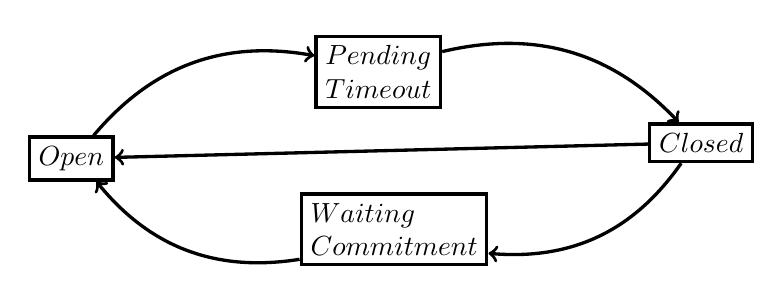
\begin{tikzpicture}
\begin{scope}[very thick,->]
    \path (-4,1)--(-4,0)--(0.1,0) node (commitment) [draw,align=left] {$Waiting$\\$Commitment$};
    \path  (0,0)--(4,0)--(4,1.1) node (closed) [draw] {$Closed$};
    \path (4,1)--(4,2)--(-0.1,2) node (pending) [draw,align=left] {$Pending$\\$Timeout$};
    \path (0,2)--(-4,2)--(-4,0.9) node (open) [draw] {$Open$};
    \draw [->,draw](closed) to [left] node  {} (open);
    \draw [->,draw](commitment) to [bend left] node {} (open);
    \draw [->,draw](open) to [bend left] node [align=center] {} (pending);
    \draw [->,draw](pending) to [bend left] node {} (closed); 
    \draw [->,draw](closed) to [bend left] node {} (commitment); 


    
  \end{scope}
\end{tikzpicture}
\end{center}
\label{fig:channel workflow}
    \caption{Channel workflow}
\end{figure}
\begin{comment}
  \draw [->,draw](commitment) to [bend left] node {\textsf{fund()}} (open);
    \draw [->,draw](open) to [bend left] node [align=center] {\textsf{initiateChannelClosure()}} (pending);
    \draw [->,draw](pending) to [bend left] node {\textsf{finalizeChannelClosure()}} (closed);  
\end{comment}

       


\subsection{On-chain Commitment}

HOPR uses a commitment scheme to deposit values on-chain and reveal them once a node redeems an incentive for relaying packets. This comes with the benefit that the redeeming party discloses a secret that is unknown to the issuer of the incentive until it is claimed on-chain. The $opening$ and the $response$ to the PoR challenge are then used by the smart contract to determine whether the ticket has been or not.

\begin{defnsub}
    % Currently leaving out further details such as unconditionally/computationally binding / hiding
    A commitment scheme $Cm = (\mathsf{Commit}, \mathsf{Open})$ is a protocol between two parties, $A$ and $B$, that gives $A$ the opportunity to store a value $comm = \mathsf{Commit}(x)$ at $B$. The value $x$ stays unknown to $B$ until $A$ decides to reveal it to $B$.

    \noindent\textbf{Hiding:} A commitment scheme is called \textbf{hiding} if it is infeasible for an adversary $\mathsf{Adv}$ to recover $x$ from $comm$.

    \noindent\textbf{Binding:} A commitment scheme is called \textbf{binding} if it is infeasible for an adversary $\mathsf{Adv}$ to find a value $x'$ with $x \neq x'$ such that $\mathsf{Open}(cm, x') \neq \bot$.
\end{defnsub}

\subsubsection{Setup phase}

Once a node engages with another node in a payment channel and lock funds within that channel, it derives a master key $comm_0$ from its private key and uses it to create an iterated commitment $comm_i$ such that for every $i \in \mathbb{N}_0$ and $i > 0$ it holds that $$ \mathsf{Open}(comm_{i}, comm_{i-1}) = \top $$

The iterated commitment is computed as $comm_n = hash^n(comm_0)$ where $\mathsf{hash}$ is a preimage-resistant hash function and $comm_0$ is derived as: $$ comm_0 = \mathsf{hash}(privKey, chainId, contractAddr, channelId, channelEpoch)$$

The master key is supposed to be pseudo-random such that all intermediate commitments $comm_{i}$ for $i \in \mathbb{N}_0$ and $0 < i \le n$ are indistinguishable for the ticket issuer from random numbers of the same length. This is necessary in order to ensure that the ticket issuer is unable to determine whether a ticket is a win or not when issuing the ticket. This makes it infeasible for the ticket issuer to tweak the challenge to such that it cannot be a win.

When dispatching a transaction that opens the payment channel, the commitment $comm_n$ is stored in the channel structure in the smart contract and the smart contract will force the ticket recipient to reveal $comm_{n-1}$ when redeeming a ticket issued in this channel.

The number of iterations $n$ can be chosen as a constant and should reflect the number of tickets a node intends to redeem within a channel.

\subsubsection{Opening phase}

In order to redeem a ticket, a node has to reveal the opening to the current commitment $comm_i$ that is stored in the smart contract for the channel. Since the opening $comm_{i-1}$ allows the ticket issuer to determine whether a ticket is going to be a win, the ticket recipient should keep $comm_{i-1}$ until it is used to redeem a ticket.

Tickets lead to a win if $\mathsf{hash}( t_h, r, comm_{i-1} ) < P_w$ where $t_h=\mathsf{hash}(t)$ and $\mathsf{Open}(comm_i, comm_{i-1}) = \top$. Since $comm_{0}$ is known to the ticket recipient, the ticket recipient can compute the opening as $comm_{n-1} = \mathsf{hash}^{n-1}(comm_0)$.

Once redeeming a ticket, the smart contract verifies that $$\mathsf{Open}(comm_i, comm_{i-1}) = \top$$ and sets $channel.comm[redeemer] \leftarrow comm_{i-1}$. Hence next time, the node redeems a ticket, it has to reveal $comm_{i-2}$.

In addition, each node is granted the right to reset the commitment to a new value which is necessary especially once a node reveals $comm_0$ and therefore is with high probability unable to compute a value $r$ such that $$\mathsf{Open}(comm_0,r) \neq \bot$$.

Since this mechanism can be abused by the ticket recipient to tweak the entropy that is used to determine whether a ticket is a win or not, the smart contract keeps track on resets of the on-chain commitment and sets $$channel.ticketEpoc[redeemer] \leftarrow channel.ticketEpoc[redeemer] + 1$$ and thereby invalidates all previously unredeemed tickets.




\subsection{Proof Of Relay}

HOPR incentivizes packet transformation and delivery using a mechanism called “Proof-Of-Relay”.
This mechanism guarantees that nodes relay services are verifiable.
\paragraph{Construction}
\begin{itemize}
    \item Every packet is sent together with a ticket (check ticket section).
    \item Each ticket contains a challenge.
    \item The validity of a ticket can only be checked on reception of the packet but the on-chain logic enforces a solution to the challenge stated in the ticket (check ticket section).
\end{itemize}

\subsubsection{Challenge}
$(A)$ creates a shared secret $s_i$ with all the relay nodes in the channel (B-C-D-Z) by using an offline version of the Diffie-Hellman key exchange. This shared key is a session key that's generated from the master DH key sphinx key.
    \\~\\ The shared secret $s_i$ is used as a seed for a PRG (Pseudo Random Generator) to create secret shares $s_i^{(0)},s_i^{(1)}$ for each node along the route.
    Relayers compute $s_i^{(0)}$ and get $s_{i+1}^{(1)}$ from the next downstream node.
    \newline The sender $(A)$ provides a hint to the expected value $s_{i+1}^{(1)}$ that a node $n_i$ is expected to get from the next downstream node.
    The value “hint” or $H$ is computed as 
    \begin{align}  
        H_i&=s_{i+1}^{(1)}*G
         \end{align}
    where $*$ is the curve multiplication operation and $G$ is a generator of the curve (the same used in the sphinx section). 
    \newline The hint for party $n_i$ is used to check whether the returned value $s_{i+1}'^{(1)}$ matches the promised value $s_{i+1}^{(1)}$ by checking whether $hint_i$ equals $s_{i+1}'^{(1)}*G$. 
   \\The sender $(A)$ also creates a challenge $T_{c_i}$ such that 
   \begin{align}  
    T_{c_i}&=(s_i^{(0)}+s_{i+1}^{(1)})*G
     \end{align}
   Since “Proof-Of-Relay” is used to make the relay services of nodes verifiable, it is the duty of each node to check that given challenges are derivable from the given and the expected information.
Packets with inappropriate challenges should be dropped as they might not lead to winning tickets.
\begin{comment}
 \begin{figure}[H]
    \centering
    \begin{tabular}{| m{2em} | m{15em} | m{2em} |}
        \hline
        $\alpha$ & $\beta$                   & $\gamma$ \\
                 & \begin{tabular}{| c m{2em} | m{3em} | m{6em} |}
            \hline
            \multicolumn{2}{| c |}{$Y_B$} & $hint_B$                 & $challenge_{BC}$ \\
            \hline
            \multicolumn{2}{| c |}{$Y_C$} & $hint_C$                 & $random$         \\
            \hline
            \multicolumn{2}{| c |}{$Y_D$} & $hint_D$                 & $random$         \\
            \hline
            End                           & \multicolumn{3}{| l |}{}                    \\
            \hline
        \end{tabular} &          \\[3em]
        \hline
    \end{tabular}
    \caption{SPHINX with PoR}
    \label{fig:SPHINX with PoR}
\end{figure}
\end{comment}
